% =============================================================================
% SECTION 7 -- TOOLS YOU SHOULD LEARN
% =============================================================================

\section{Tools You Should Learn}
\subsection{Git \& Friends}

% ---------------------------------------------------------------------------
% 7.1  personal website? git!
% ---------------------------------------------------------------------------
\begin{frame}{How many of you have a personal website?}{hands up!}
    \begin{center}
        \glowtitle[neonyellow]{Hands up!}
    \end{center}
    \pause
    \begin{columns}
        \begin{column}{0.55\textwidth}
            {\small\color{fgwhite} Want one? Host it free on:}
            \begin{center}
                \begin{tabular}{ccc}
                    \logopic[1.0cm]{github}  & \logopic[1.0cm]{gitlab}  & \logopic[1.0cm]{codeberg}\\[0.1em]
                    {\tiny GitHub}           & {\tiny GitLab}           & {\tiny Codeberg}\\
                \end{tabular}
            \end{center}
            {\small Underlying tool: \glow{git}. You need to learn git.}
            \onslide<3->{\begin{tcolorbox}[darkstyle,title={\tiny \$ your first repo}]
                {\ttfamily\tiny
                \textcolor{neongreen}{\$} git init\\[-0.15em]
                \textcolor{neongreen}{\$} git add .\\[-0.15em]
                \textcolor{neongreen}{\$} git commit -m "my first website"\\[-0.15em]
                \textcolor{neongreen}{\$} git push origin main}
            \end{tcolorbox}}
        \end{column}
        \begin{column}{0.4\textwidth}
            \onslide<4->{\begin{center}
                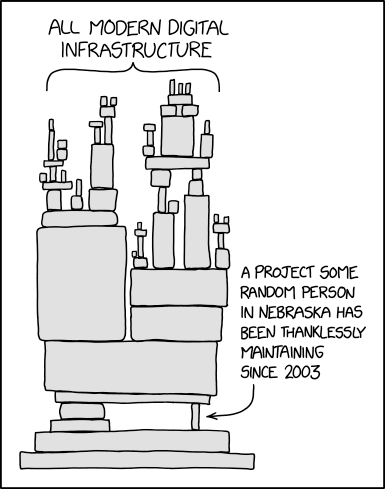
\includegraphics[height=4.2cm]{assets/img/xkcd_dependency.png}\\[0.1em]
                {\tiny\color{softgray} xkcd 2347: Dependency --- everyone runs on git, eventually}
            \end{center}}
        \end{column}
    \end{columns}
\end{frame}

% ---------------------------------------------------------------------------
% 7.2  latex & overleaf
% ---------------------------------------------------------------------------
% ---------------------------------------------------------------------------
% 7.2  github project overview (image only)
% ---------------------------------------------------------------------------
\begin{frame}{GitHub, in action}{the project overview}
    \begin{center}
        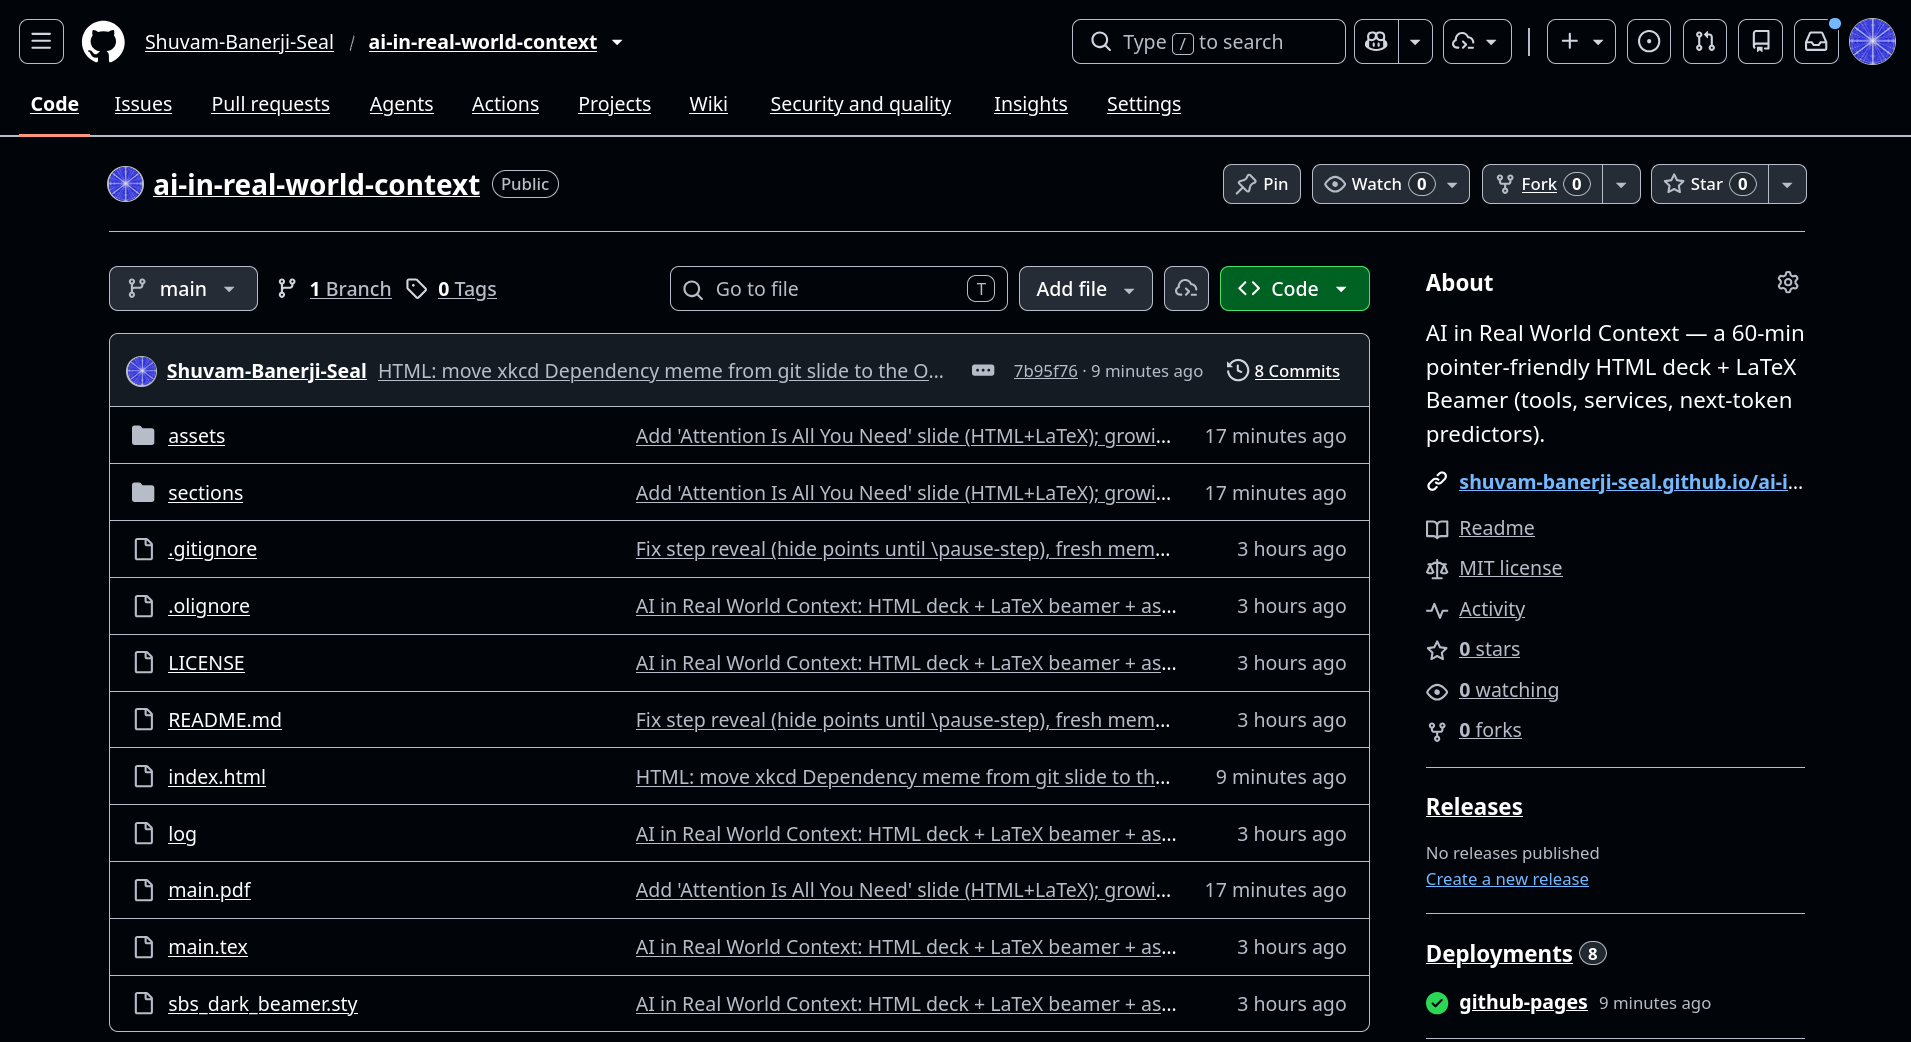
\includegraphics[height=6.2cm]{assets/img/github_project_overview_screenshot.png}
    \end{center}
\end{frame}

\subsection{\texorpdfstring{\LaTeX{} \& Overleaf}{LaTeX and Overleaf}}

\begin{frame}{Overleaf \& \LaTeX}{assignments, thesis, projects}
    \begin{columns}
        \begin{column}{0.42\textwidth}
            \begin{center}
                \begin{tabular}{cc}
                    \logopic[1.5cm]{overleaf} & \logopic[1.5cm]{latex}\\[0.1em]
                    {\tiny Overleaf}          & {\tiny \LaTeX}\\
                \end{tabular}
            \end{center}
        \end{column}
        \begin{column}{0.52\textwidth}
            \pause\begin{itemize}[<+->]
                \item PDFs: assignments, thesis, projects --- all \glow{\LaTeX}.
                \item You type text + commands; the machine typesets beauty.
                \item Overleaf = \LaTeX{} in your browser, zero install.
            \end{itemize}
            \onslide<5->{\begin{infobox}[fun fact]
                {\small Heck --- even this presentation is made using \LaTeX.\\ You are literally reading typeset tokens.}
            \end{infobox}}
        \end{column}
    \end{columns}
\end{frame}

% ---------------------------------------------------------------------------
% 7.3  overleaf project view (image only)
% ---------------------------------------------------------------------------
\begin{frame}{Overleaf, in action}{the project view}
    \begin{center}
        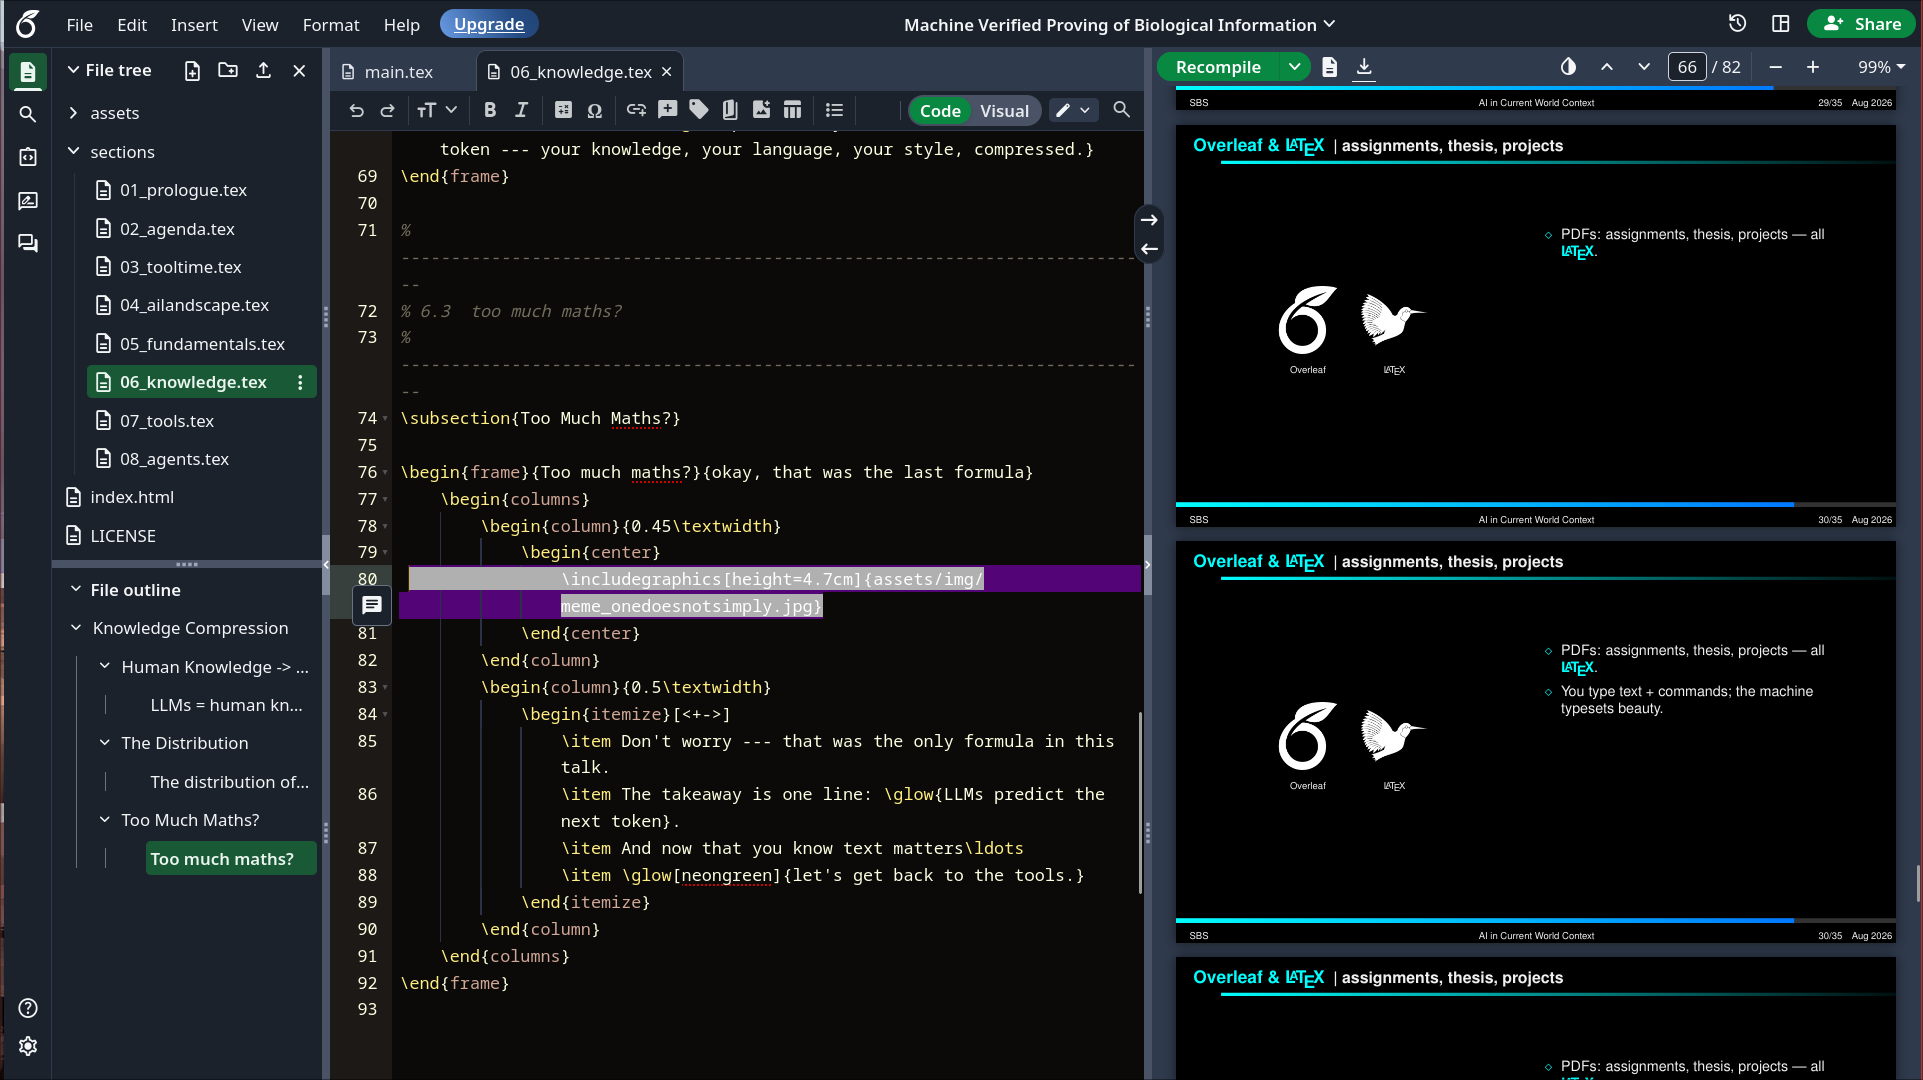
\includegraphics[height=6.2cm]{assets/img/overleaf_projectview_image.png}
    \end{center}
\end{frame}

% ---------------------------------------------------------------------------
% 7.4  would you do it by yourself?
% ---------------------------------------------------------------------------
\subsection{Do It Yourself?}

\begin{frame}{Would you do it by yourself?}{now that everything is text}
    \begin{columns}
        \begin{column}{0.52\textwidth}
            {\small So now I've asked you to build a website and write an assignment.}
            \pause\begin{itemize}[<+->]
                \item Would you want to do it all \glow{by yourself}?
                \item Remember: everything here is \glow[neongreen]{text}.
                \item And text is exactly what AI agents are good at.
            \end{itemize}
            \onslide<5->{\begin{successbox}[the pitch]
                {\small Use \glow{agentic tools} --- like the ones I'm about to show.}
            \end{successbox}}
        \end{column}
        \begin{column}{0.44\textwidth}
            \begin{center}
                
\includegraphics[height=5.3cm]{assets/img/meme_drake.png}
            \end{center}
        \end{column}
    \end{columns}
\end{frame}
